\section{Introduction}
\addcontentsline{toc}{chapter}{Introduction}


Ce livre a pour but de vous faire faire des mathématiques. On commence par du calcul mental afin d’échauffer l’esprit. Oui, même au XXI\up{e} siècle, alors que nous avons des calculatrices, des ordinateurs, des téléphones et même des intelligences artificielles, il est encore utile d’exercer son cerveau sur ce genre de tâches. Loin de moi l’idée de vous prendre pour des calculateurs prodiges, ni d’essayer de vous entraîner à le devenir : je n’en suis pas un, et j’aurais du mal à vous aider pour ce genre de compétitions. Mais, de la même façon que les humains n’ont pas cessé de marcher et de courir après l’invention de la voiture, de l’ascenseur et des autres moyens de transport, il en va de même pour l’exercice cérébral. Sans être médecin, il me semble que le bon sens nous dicte que, si l’on reste assis sur le canapé à manger de la malbouffe sans faire de sport, il y a de gros risques de rencontrer des problèmes de surpoids et de santé en général. L’exercice cérébral est une gymnastique de l’esprit : c'est une \urlnote{hygiène mentale}{https://www.youtube.com/watch?v=qrA5HgFIjJE}.

Néanmoins, il serait vain — et surtout ennuyeux — de se cantonner aux calculs. L’activité mathématique est bien plus riche que cela. Il ne s’agit pas de comptabilité. Même si l’arithmétique et le calcul algébrique restent des outils cruciaux dans l’architecture des mathématiques, les maths ne se résument pas à des calculs. D’un autre côté, oublier cet aspect serait une carence aussi flagrante que celle d’un sportif de haut niveau (footballeur, nageur, judoka… choisissez votre sport favori) qui ne ferait pas de musculation. Les sportifs font de la musculation parce que leurs muscles sont leurs outils pour accomplir leur art. En mathématiques, c’est pareil : les calculs et la capacité à les conduire sont utiles pour résoudre des problèmes mathématiques.

Ce livre s’articule en trois parties principales, en plus de cette introduction.

La première partie doit être faite par tous les lecteurs en guise d’échauffement. Il s’agit de calculs \frquote{\textit{purs et durs}}, de niveau primaire. En effet, l’école primaire a pour but de faire acquérir la maîtrise des quatre opérations de l’arithmétique de base, à savoir : addition, soustraction, multiplication et division. Cela peut paraître simple, mais derrière ces \frquote{\textit{simples}} opérations se cachent les structures algébriques que nous aborderons dans un prochain ouvrage consacré à l’enseignement supérieur.

Dans la seconde partie, on passe au niveau collège, en ajoutant des calculs de carrés, des programmes de calculs, le calcul littéral, les liens entre géométrie et calcul, et des probabilités de base en termes de rapports d’aires de figures élémentaires.

Enfin, dans la troisième partie, on passe au niveau lycée : configurations de nombres, vecteurs, statistiques et situations concrètes. Mais les choses sont présentées avec un vocabulaire et des connaissances accessibles à un collégien. 

Le souhait de cet ouvrage est de fournir des exercices faisables directement, sans avoir à \textit{réviser le cours}. Trop souvent aujourd’hui, les élèves sont traumatisés par la crainte de ne pas connaître \frquote{\textit{la phrase du cours}}, comme s’il s’agissait d’une incantation magique. Aucun cours de mathématiques n’est tombé du ciel, telles les tables de la Loi. L’activité mathématique s’est développée au cours des siècles à travers des problèmes qui, une fois résolus, ont donné lieu à des généralisations, lesquelles sont ensuite devenues des cours. Alors bien sûr, on ne peut pas se permettre le luxe de tout redémontrer à partir de zéro, sinon chaque génération aurait à refaire tout ce qu’a fait la précédente. Néanmoins, il me semble beaucoup plus intéressant, et surtout utile et efficace, de s’exercer d’abord ; et, à force de pratique, le cours pourra alors être vu comme quelque chose d’intéressant… un nouveau genre d’exercice.

Ma critique première est que les enseignements primaires et secondaires (surtout primaire et collège) manquent cruellement de démonstrations (alors que des démonstrations géométriques sont accessibles très tôt comme par exemple la \urlnote{démonstration de la 1\up{ère} identité remarquable}{https://youtu.be/IL55ftyJQHI} ), au profit d’un apprentissage par cœur dénué de raisonnement et de réflexion, destiné à créer des \frquote{\textit{automatismes}}. À l’époque de l’intelligence artificielle, il me semble d’autant plus absurde de vouloir former des générations d’automates, déjà dépassés par les véritables automates. Nous, humains, faisons des erreurs et avons la capacité d’apprendre de nos erreurs. C’est précisément pour cette raison qu’il faut cultiver l’art de se tromper intelligemment.

L’art de se tromper intelligemment signifie prendre le risque de pousser un raisonnement jusqu’à son terme, pour se rendre compte s’il fonctionne ou non. Comprendre signifie prendre un risque : sans prise de risque, vous ne pourrez jamais comprendre ; sans erreur, vous ne pourrez jamais comprendre.

Ici, tous les exercices sont corrigés, donc vous pouvez les faire en toute honnêteté, en prenant véritablement le risque de vous tromper. De plus, pour la plupart des exercices (en dehors de ceux de calculs purs), il y a souvent plusieurs façons de les résoudre. Il ne faut donc pas chercher à mémoriser les corrections. Les exercices sont presque tous originaux ou des adaptations de classiques.

\newpage

Pour toutes remarques, suggestions, ou demandes d'aide personnelles merci de remplir \urlnote{ce formulaire}{https://forms.gle/x7fAce7GqiJAGbsC7} : \url{https://forms.gle/x7fAce7GqiJAGbsC7}. Si vous souhaitez obtenir la version numérique de ce livre c'est aussi ce même formulaire qu'il faut remplir afin que nous puissions entrer en contact.

\newpage 

\subsection{Origine étymologique du mot calcul}

\begin{wrapfigure}[5]{l}{0.4\textwidth} % 8 = lignes occupées, l = à gauche
    \vspace{-0.75cm} % remonte l’image pour l’aligner avec la 1ère ligne du texte
    \includegraphics[width=0.4\textwidth]{../images/Cailloux.jpeg}
    %\caption{}
\end{wrapfigure}

Le mot \frquote{calcul} vient du latin \textbf{\textit{calculus}}, qui signifiait littéralement \frquote{petit caillou}. Ce terme dérive de \textbf{\textit{calx}}, \textbf{\textit{calcis}} (chaux, pierre calcaire). Les Romains utilisaient effectivement de petits cailloux ou jetons pour effectuer leurs opérations arithmétiques sur l'abaque, d'où cette étymologie concrète qui reflète une pratique réelle. 

\newpage 

\subsection{Premières traces de calculs}

Les plus anciennes traces de calculs remontent à la préhistoire :

\vspace{.5cm}



\textsc{Os d'Ishango} (République démocratique du Congo, ~20 000 ans) : 

\vspace{.2cm}

\begin{wrapfigure}[8]{l}{0.22\textwidth} % 8 = lignes occupées, l = à gauche
    \vspace{-0.65cm} % remonte l’image pour l’aligner avec la 1ère ligne du texte
    \includegraphics[width=0.22\textwidth]{../images/Os-Ishango.jpeg}
    %\caption{Os d'Ishango}
\end{wrapfigure}

Les os d'Ishango, également appelés bâtons d'Ishango, sont considérés comme le plus ancien outil de calcul jamais mis au jour. Ils ont été découverts au sein de vestiges archéologiques découverts dans l'ancien Congo belge. Le site est daté de plus de 20 000 ans. Selon certains auteurs, il pourrait s'agir de la plus ancienne attestation de la pratique de l'arithmétique dans l'histoire de l'humanité. Ils ont été considérés, dans un premier temps, comme des bâtons de comptage. 


\newpage

\textsc{ Jetons d'argile mésopotamiens} (~8000-3000 av. J.-C.) : 

\vspace{.2cm}

\begin{wrapfigure}[7]{l}{0.25\textwidth} % 8 = lignes occupées, l = à gauche
    \vspace{-0.6cm} % remonte l’image pour l’aligner avec la 1ère ligne du texte
    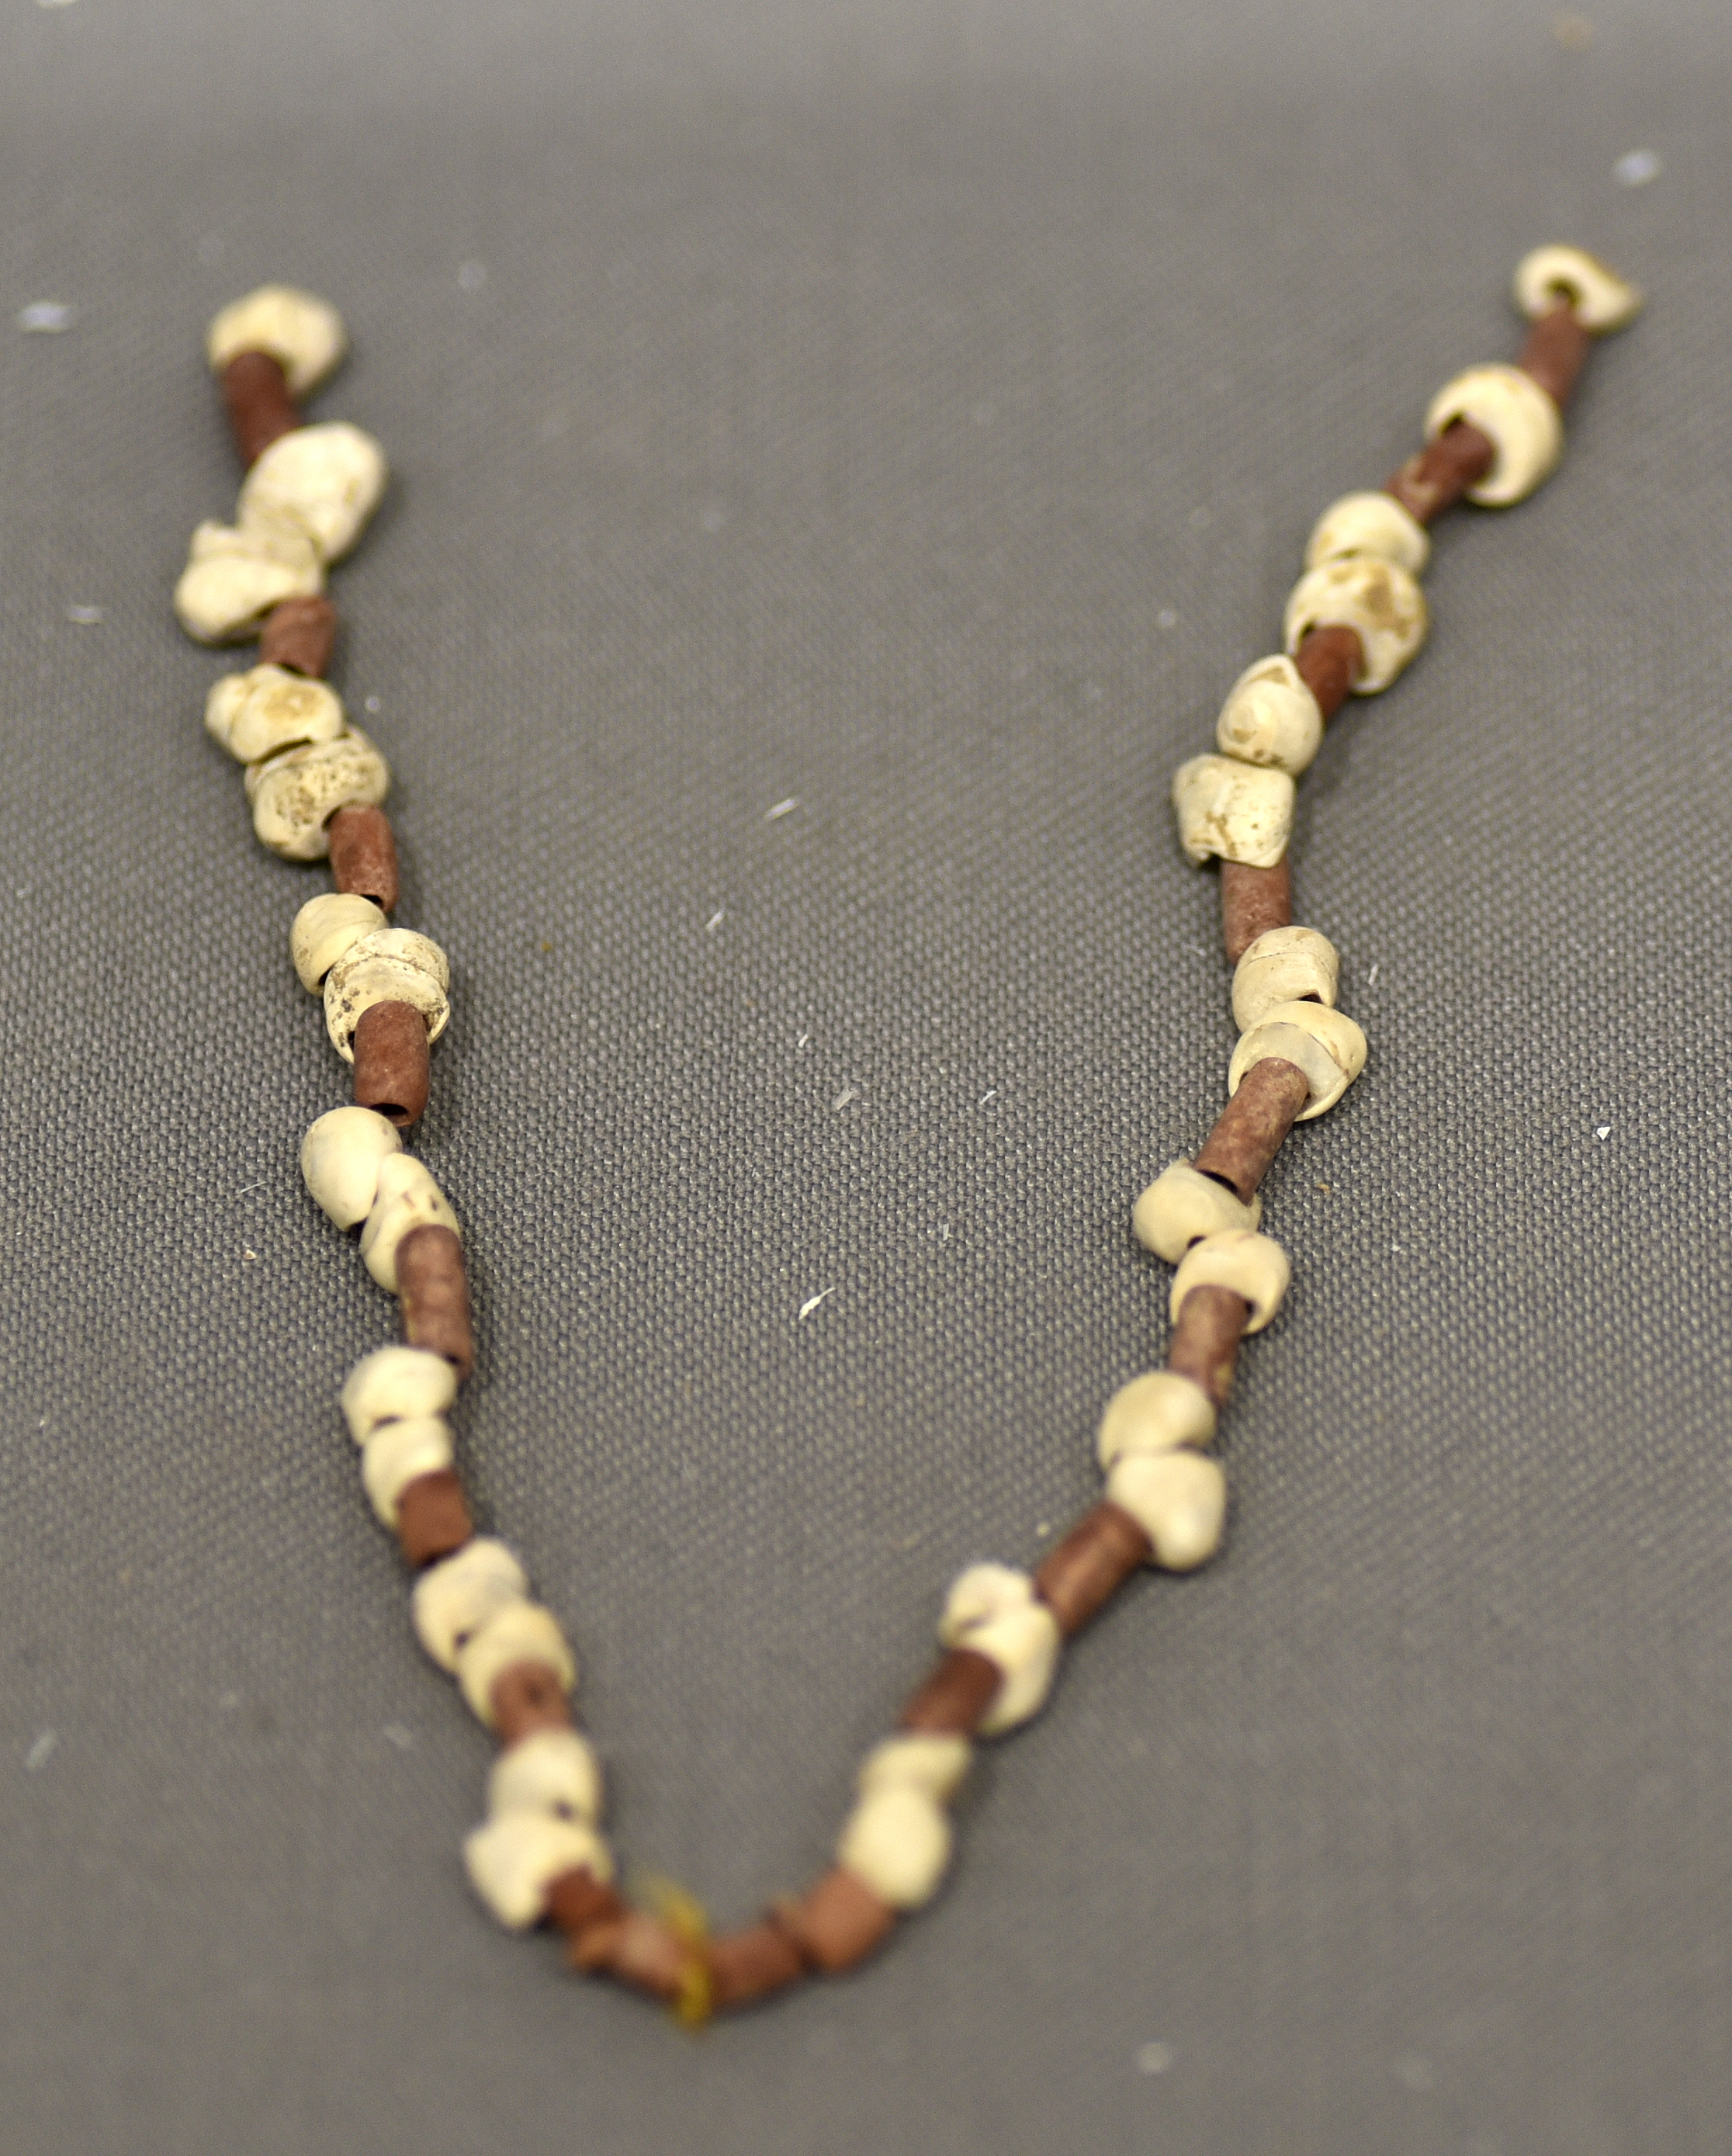
\includegraphics[width=0.25\textwidth]{../images/collier7800.jpg}
    %\caption{}
\end{wrapfigure}

Ces petits objets en forme de cônes, sphères ou disques servaient à compter les biens (bétail, céréales) avant l'invention de l'écriture. Les jetons d'argile mésopotamiens ont joué un rôle important dans le développement des systèmes de comptabilité et de commerce dès 8000 avant J.-C. Ces objets, dont la forme variait en fonction de l'objet qu'ils représentaient, étaient utilisés pour désigner et quantifier des marchandises.

\newpage


\textsc{ Tablettes cunéiformes babyloniennes} (~3000 av. J.-C.) : 

\vspace{.2cm}

\begin{wrapfigure}[5]{l}{0.55\textwidth} % 8 = lignes occupées, l = à gauche
    \vspace{-0.75cm} % remonte l’image pour l’aligner avec la 1ère ligne du texte
    \includegraphics[width=0.55\textwidth]{../images/Proto-cuneiform-sexagesimal.pdf}
    %\caption{}
\end{wrapfigure}

Les premières traces écrites de calculs arithmétiques, avec un système sexagésimal (base 60) encore utilisé aujourd'hui pour mesurer le temps (1 heure = 60 minutes, 1 minute = 60 secondes, \dots ) et les angles (60 minutes = 1 degré).

\newpage

\textsc{ Papyrus de Rhind} (~2000 av. J.-C.):

\vspace{.2cm}

\begin{wrapfigure}[7]{l}{0.5\textwidth} % 8 = lignes occupées, l = à gauche
    \vspace{-0.75cm} % remonte l’image pour l’aligner avec la 1ère ligne du texte
    \includegraphics[width=0.5\textwidth]{../images/Rhind-Papyrus.jpg}
    %\caption{}
\end{wrapfigure}

Le papyrus Rhind, copié par Ahmès (Deuxième Période intermédiaire), synthétise les maths égyptiennes. Acheté par Rhind en 1858 à Louxor, il est au British Museum depuis 1865. Ce rouleau de 5 m (87 problèmes) couvre arithmétique, algèbre et géométrie, inspiré du Moyen Empire (2000 av. J.-C.). Son écriture hiératique en fait un document unique.


\newpage 


\subsection{Premières techniques de calcul}

\textsc{ L'abaque :} 

\vspace{.35cm}

\begin{wrapfigure}[7]{l}{0.55\textwidth} % 8 = lignes occupées, l = à gauche
    \vspace{-0.75cm} % remonte l’image pour l’aligner avec la 1ère ligne du texte
    \includegraphics[width=0.55\textwidth]{../images/Abacus.png}
    %\caption{}
\end{wrapfigure}

Apparu vers 2700-2300 av. J.-C. en Mésopotamie, puis perfectionné par les Grecs et les Romains. Il permettait d'effectuer les quatre opérations fondamentales en déplaçant des jetons sur des lignes ou dans des colonnes.


\newpage

\textsc{ Le système décimal positionnel :} 

\vspace{.35cm}

\begin{wrapfigure}[12]{l}{0.6\textwidth} % 8 = lignes occupées, l = à gauche
    \vspace{-0.75cm} % remonte l’image pour l’aligner avec la 1ère ligne du texte
    \includegraphics[width=0.6\textwidth]{../images/Numeration.png}
    %\caption{}
\end{wrapfigure}

Le système de numération indo-arabe est un système de numération de base dix employant une notation positionnelle et dix chiffres, allant de zéro à neuf, dont le tracé est indépendant de la valeur représentée. Dans ce système, la représentation d'un nombre correspond à son développement décimal. Le système doit son nom au fait qu'il est apparu en Inde et qu'il est parvenu en Europe par l'intermédiaire de mathématiciens et comptables de langue arabe. La variante graphique la plus répandue sont les chiffres utilisés en Europe, communément appelés chiffres arabes. Ce système tend aujourd’hui à s’imposer dans le monde.

\newpage

\textsc{ Les bâtons de Napier (1617) :} 

\vspace{.35cm}

\begin{wrapfigure}[8]{l}{0.45\textwidth} % 8 = lignes occupées, l = à gauche
    \vspace{-0.75cm} % remonte l’image pour l’aligner avec la 1ère ligne du texte
    \includegraphics[width=0.45\textwidth]{../images/batons-napier.jpg}
    %\caption{}
\end{wrapfigure}

Le bâton de Napier, ou réglette de Neper est un abaque facilitant le calcul des produits, quotients, puissances et racines, inventé par le mathématicien écossais John Napier (en français Neper) en 1617.

L'abaque est constitué d'un plateau à rebord sur lequel peuvent être placées des réglettes gravées. Le bord gauche du plateau est gravé lui aussi, divisé en neuf cases numérotées de 1 à 9. Les dix types de réglettes, qui ont donné leur nom à l'ensemble du dispositif, étaient originellement en os, d'où le nom anglais de \textit{Napier's bones}. Elles sont divisées en neuf cases. La case supérieure porte un nombre de 0 à 9. Les huit autres cases sont divisées en deux par un trait diagonal.

\newpage

\textsc{ La pascaline (1642) :} 

\vspace{.35cm}

\begin{wrapfigure}[5]{l}{0.4\textwidth} % 8 = lignes occupées, l = à gauche
    \vspace{-0.75cm} % remonte l’image pour l’aligner avec la 1ère ligne du texte
    \includegraphics[width=0.4\textwidth]{../images/pascaline.jpg}
    %\caption{}
\end{wrapfigure}


La pascaline, initialement dénommée machine d’arithmétique puis roue pascaline, est une calculatrice mécanique inventée par Blaise Pascal et considérée comme la première machine à calculer. 


\newpage

\subsection{Les premières traces de géométrie}

Si les Grecs sont souvent vus comme les fondateurs de la géométrie en tant que science, de nombreuses connaissances en géométrie ont émergé bien avant eux, notamment vers 3000 av. J.-C., en Égypte ancienne, en Mésopotamie et dans l'Inde antique, pour répondre à des besoins pratiques en agriculture, astronomie, architecture et topographie.

\vspace{.5cm}



\textsc{Manuscript de Bakhshali} (Civilisation de la vallée de l'Indus) : 

\vspace{.2cm}

\begin{wrapfigure}[6]{l}{0.5\textwidth} % 6 = lignes occupées, l = à gauche
    \vspace{-0.65cm} % remonte l’image pour l’aligner avec la 1ère ligne du texte
    \includegraphics[width=0.5\textwidth]{../images/Bakhshali_manuscript.jpg}
    %\caption{Os d'Ishango}
\end{wrapfigure}

La civilisation de la vallée de l'Indus, attestée dès environ -3300, livre les premiers indices d'une activité mathématique en Inde. Les découvertes effectuées à Harappa, Mohenjo-daro et dans leur environnement révèlent un système de poids et mesures précis et décimal datant d’environ 2600 avant J.-C., une technologie de fabrication de briques basée sur des proportions rigoureuses, ainsi qu’une attention aux formes géométriques.


\newpage


\textsc{Tablette babylonienne YBC 7289} (Babylone) : 

\vspace{.2cm}

\begin{wrapfigure}[10]{l}{0.5\textwidth} % 10 = lignes occupées, l = à gauche
    \vspace{-0.65cm} % remonte l’image pour l’aligner avec la 1ère ligne du texte
    \includegraphics[width=0.5\textwidth]{../images/Ybc7289.jpg}
    %\caption{Os d'Ishango}
\end{wrapfigure}

La tablette YBC 7289 a probablement été rédigée par un scribe babylonien de la première dynastie, entre 1900 et 1600 avant J.-C. Elle aurait été écrite dans le sud de l’actuel Irak, vraisemblablement par un apprenti utilisant des valeurs tirées d’une liste connue. De forme ronde et compacte (8 à 12 cm environ), elle était facile à tenir en main. 

La suite de nombres est à interpréter de la façon suivante : 
\begin{align*}
1 + \dfrac{24}{60} + \dfrac{51}{60^2} + \dfrac{10}{60^3} &\simeq \sqrt{2}\\
42 + \dfrac{25}{60} + \dfrac{35}{60^2} &\simeq 30\sqrt{2}
\end{align*}

\newpage


\textsc{Papyrus de Moscou} (Civilisation Egyptienne) : 

\vspace{.2cm}

\begin{wrapfigure}[7]{l}{0.65\textwidth} % 7 = lignes occupées, l = à gauche
    \vspace{-0.65cm} % remonte l’image pour l’aligner avec la 1ère ligne du texte
    \includegraphics[width=0.65\textwidth]{../images/papyrus-moscou.jpg}
    %\caption{Os d'Ishango}
\end{wrapfigure}

Écrit vers 1850 av. J.-C., pendant la XIe dynastie, le papyrus de Moscou est un exemple ancien d’étude mathématique utilisant le système unaire. Long d’environ 5,40 mètres et large de 4 à 7 cm, il contient 25 problèmes résolus, dont certains portent sur la surface d’une demi-sphère et le volume d’une pyramide tronquée.


\newpage


\textsc{Les Neuf Chapitres sur l'art mathématique} (Civilisation Chinoise après les Grecs) : 

\vspace{.2cm}

\begin{wrapfigure}[10]{l}{0.35\textwidth} % 10 = lignes occupées, l = à gauche
    \vspace{-0.65cm} % remonte l’image pour l’aligner avec la 1ère ligne du texte
    \includegraphics[width=0.35\textwidth]{../images/9chap.jpg}
    %\caption{Os d'Ishango}
\end{wrapfigure}

Les Neuf Chapitres sur l’art mathématique forment un ouvrage chinois anonyme compilé entre le IIe et le Ier siècle av. J.-C., au début de la dynastie Han. Reprenant des textes antérieurs, il propose une approche méthodique des mathématiques à travers des techniques générales de résolution de problèmes. Connu grâce aux copies des scribes puis à l’imprimerie, il fut commenté notamment par Liu Hui en 263.


\newpage

